% 
% Annual Cognitive Science Conference
% Sample LaTeX Paper -- Proceedings Format
% 

% Original : Ashwin Ram (ashwin@cc.gatech.edu)       04/01/1994
% Modified : Johanna Moore (jmoore@cs.pitt.edu)      03/17/1995
% Modified : David Noelle (noelle@ucsd.edu)          03/15/1996
% Modified : Pat Langley (langley@cs.stanford.edu)   01/26/1997
% Latex2e corrections by Ramin Charles Nakisa        01/28/1997 
% Modified : Tina Eliassi-Rad (eliassi@cs.wisc.edu)  01/31/1998
% Modified : Trisha Yannuzzi (trisha@ircs.upenn.edu) 12/28/1999 (in process)
% Modified : Mary Ellen Foster (M.E.Foster@ed.ac.uk) 12/11/2000
% Modified : Ken Forbus                              01/23/2004
% Modified : Eli M. Silk (esilk@pitt.edu)            05/24/2005
% Modified : Niels Taatgen (taatgen@cmu.edu)         10/24/2006
% Modified : David Noelle (dnoelle@ucmerced.edu)     11/19/2014
% Modified : Roger Levy (rplevy@mit.edu)     12/31/2018



%% Change "letterpaper" in the following line to "a4paper" if you must.

\documentclass[10pt,letterpaper]{article}
\usepackage{hyperref}

\usepackage{cogsci}

\cogscifinalcopy % Uncomment this line for the final submission 


\usepackage{pslatex}
\usepackage{apacite}
\usepackage{tikz}
\usepackage{float} % Roger Levy added this and changed figure/table
                   % placement to [H] for conformity to Word template,
                   % though floating tables and figures to top is
                   % still generally recommended!

%\usepackage[none]{hyphenat} % Sometimes it can be useful to turn off
%hyphenation for purposes such as spell checking of the resulting
%PDF.  Uncomment this block to turn off hyphenation.


%\setlength\titlebox{4.5cm}
% You can expand the titlebox if you need extra space
% to show all the authors. Please do not make the titlebox
% smaller than 4.5cm (the original size).
%%If you do, we reserve the right to require you to change it back in
%%the camera-ready version, which could interfere with the timely
%%appearance of your paper in the Proceedings.
\def\arraystretch{1.15}%  1 is the default, change whatever you need


\title{Errorless irrationality: removing error-driven components from the inverse base-rate effect paradigm}
 
\author{{\large \bf Lenard Dome (lenarddome@gmail.com)} \\
  Brain Research and Imaging Centre \\
  University of Plymouth, Research Way, Plymouth, PL6 8BU
  \AND {\large \bf Andy J. Wills (andy.wills@plymouth.ac.uk)} \\
  Brain Research and Imaging Centre \\
  University of Plymouth, Research Way, Plymouth, PL6 8BU}


\begin{document}

\maketitle

\begin{abstract}
Include no author information in the initial submission, to facilitate
blind review.

\textbf{Keywords:} 
irrationality; prediction error; inverse base-rate effect; categorization; contingency learning
\end{abstract}


\section{Introduction}

The \textit{inverse base-rate effect} \cite<IBRE, >{medin1988problem} is an irrational tendency in humans to overweigh rare events when faced with ambiguity.
In a traditional design, people learn to categorise two overlapping sets of features under two distinct labels.
These sets share a single feature, A, and possess a unique feature, B and C, predictive of their respective category label.
During learning, these sets of features occur at different frequencies.
The features under the common label usually occur three times as much as features under the rare label \cite{kruschke1996base}.
Following training, people categorise features presented by themselves and un unique combinations.
People optimally label uniquely predictive features, B and C, presented individually with their respective common and rare labels.
Responses on the shared feature A also show base-rate following.
But when uniquely predictive features are paired, B and C, people tend to respond with the rare category label.
According to Classical Probability Theory, the rational response is to attribute the common label to this ambiguous compound, because it is the most frequently occuring label.
This rare bias on ambiguous combinations of BC has been observed across a different variety experimental manipulations \cite{kalish2001inverse,don2017effects,don2017effects,inkster2022effect,wills2014attention}.
For a more thorough introduction to this irrational bias, see a review by \citeA{don2021attention}.

\subsection*{Assumptions of models of the IBRE}

The most prominent theories of the inverse base-rate effect involve an attentional mechanism that drives not only learning but responding as well.
These models are EXIT \cite{kruschke2001toward}, a three-layer neural network with competitive attentional gating and a four-layer neural network with an additional rapid attentional shift \cite{paskewitz2020dissecting}.
All these explanations rely on a process that reallocates attention in response to prediction errors.
Their explanation is simple.
During learning, people learn to label the AB compound first.
They are still learning to label the AC compound, so when they make an error, attention relocates towards the uniquely predictive feature C to reduce future errors.
This results in C acquiring higher attentional salience than B.
When the ambiguous BC compound is presented, C will dominate responding, resulting in an irrational tendency to respond with the rare label.
According to these models, this irrationality results from an optimisation process that tries to reduce the errors people make.
This process results in an asymmetric representation that can be summarised as AB belongs to common, $AB \to common$, and C belongs to rare, $C \to rare$.

\subsection*{Current Study}

In this work, we intend to test this basic assumption of models of the IBRE.
In the following two experiments, we will gradually remove components from the design traditionally associated with prediction error.
Our overarching goal is to investigate whether we can still observe the IBRE, even if we experimentally remove a crucial assumption of already existing accounts.
In our first attempt, building on the observational learning condition of Experiment 2 in \citeA{johansen2007paradoxical}, we implement the canonical IBRE design with a caveat that category labels are presented in unison with features.

In our second attempt, we further remove the causal relationship between features and category labels.
The goal was to remove any design component that might affect attentional allocation or development of assymmetric representation in response to errors.
Any presumption of a causal relationship can inadvertently relocate attention in line with the direction of causality between features and labels.

\subsection*{Related Work}

To our knowledge, there is only one attempt to implement the IBRE procedure without explicit feedback.
In their Experiment 2, \citeA{johansen2007paradoxical} tried to observe the inverse base-rate effect both in a predictive-learning condition and in an observational learning condition, where category labels were presented with features at the same time to participants.
Their design involved disjoint cues (where categories shared no features in common), while the canonical design depends on a shared feature during training that facilitates attentional relocation.
This attentional tuning in turn pushes responding toward the rare label.
Their design was optimized to investigate the hypothesised asymmetric cognitive representation of the two categories.
As a result, the only instance when they observed a rare bias was when common features presented in compound during training were paired with a rare feature presented by itself during training.
This provided evidence for the asymmetric cognitive representation hypothesised to develop during training.
A simple neural-network explanation can account for this by positing that the rare feature developed stronger connections with the category label.
Compound features share the connection with the category label, so any update to these connections dissipates between them.
There is no need to relocate attention to reduce errors, therefore attention will not bias responding toward the rare label.
But stronger $C \to rare$ feature-label connections will result in a rare bias on BC compounds during the test phase.
In order to investigate the role of prediction error in response to feedback, we need to tweak their observational learning condition to conform to a more canonical implementation of the procedure.
\citeA{johansen2007paradoxical} included the result of a short pilot experiment in their Appendix.
There are no details about the procedure of this experiment, so we cannot make direct comparisons.
We will follow up on that line of investigation.

Our current study modified the canonical IBRE procedure in an attempt to remove error-driven components from the design - which includes a shared cue.
This contrasts Experiment 2 in \citeA{johansen2007paradoxical}, who tried to remove the shared cue that pushed attention towards C during training and resulted in the assymetric representation.
Here, we strictly focus on prediction error concerning behaviour.
% I will also need to include Experiment 3 listed shared cue condition


% I need to go through some studies because I think there is at least one more
The only two studies directly looking at error-driven processes in the IBRE are \citeA{inkster2022neural} and \citeA{wills2014attention}.
\citeA{wills2014attention} observed posterior selection negativity and concurrent frontal positivity for C relative to B, which gave evidence for an error-driven selective attentional learning process.
\citeA{inkster2022neural} carried out a direct investigation into brain regions underlying error-driven learning in the IBRE.
Their ROI analysis explicitly targeted areas that were hypothesised to be involved in the computation of prediction error.
They showed that these areas exhibited greater activation during the test phase for C relative to B with a presence of a shared cue during training.
Both \citeA{wills2014attention} and \citeA{inkster2022neural} gave strong evidence in support of error-driven attentional learning accounts of the IBRE.
In our study, we will look for the effect while trying to take out prediction error from the experimental design.
In contrast, they looked for the neural substrates of error-driven accounts of the effect.

\section{Experiment 1}

Below, we detail our first attempt to test whether we could observe the rare response bias without an explicit error-driven psychological mechanism.
The design component which is most likely to result in any error-driven tuning is feedback.
To remove feedback, we will present category labels with their respective features.
We retain the sequential property of the experiment, which means that participants learn about feature and category relationships on a trial-by-trial basis.
% work out how models might predict rational responding

Experiment 1 is a conceptual replication of an experiment included in the Appendix of \citeA{johansen2007paradoxical}.
The only information available is the list of test items (23), the doubled-up design (2 sets of categories and features), and the sample size.
We substantially simplified our implementation by removing the doubled-up design and reducing the number of test items to 6.

\subsection{Method}

\subsubsection*{Participants}

Participants were undergraduate students who received course credit for their participation.
We recruited 169 participants online through the SONA recruitment system.

\subsubsection*{Apparatus}

The experiment was programmed in JsPsych \cite{deleeuw2015JsPsych} to be run in a web browser.
The experiment code is avalaible at \href{https://osf.io/auwvt/?view_only=2dc8384074fa4bcf9f2e3937fdaee2b4}{OSF} and \href{https://github.com/lenarddome/ply216-observational-ibre}{GitHub}.
Participants completed the experiment on their personal computers.
The experiment did not allow the use of tablets and smartphones.

\subsubsection*{Stimuli}

Category labels corresponded with response keys and were called Disease \textbf{Z} and Disease \textbf{L}.
Category features were symptoms: fever, headache, and rash.
These physical features were randomly allocated to abstract features, A, B, and C at the beginning of each session.
Features and labels appeared in full sentences, such as '\textit{John has fever and rash, which belongs to disease Z}'.
Names were randomly drawn from a pool of male and female first names.
The list was compiled from an online repository of popular baby names\footnote[1]{The list was taken and later curated from \href{https://github.com/aruljohn/popular-baby-names}{a GitHub repository}.}.
We selected the 50 most popular male and female names from 2021.
Disease names corresponded to response keys and were randomly allocated to either the common or rare category label at the beginning of each session.

\subsubsection*{Procedure}

Table \ref{tab:abstract-exp1} summarises the abstract design of the experiment.
This design is the simplest implementation of the IBRE procedure to date.
Participants completed two phases: a training and a test phase.
In the training phase, they encountered descriptions of people, the symptoms they experienced, and their respective diseases.
These descriptions appeared in the format of '\textit{John has fever and rash, which belongs to disease Z}'.
Participants studied these examples and when they were ready to move on, they pressed the spacebar.
They needed to complete reading the description within 5 seconds.
If the 5 seconds threshold has passed, a screen appeared with the message '\textit{Please respond faster!}'.
In each training block, participants encountered 6 common diseases (common category exemplars) and 2 rare diseases (rare category exemplars).
After the second block of training, participants were given a choice.
They could either move straight to the test phase or complete another training block.
There were a maximum of 5 blocks they could complete.

In the test phase, participants judged individual symptoms and novel combinations of old symptoms, see Table \ref*{tab:abstract-exp1}.
Symptoms appeared in a sentence, such as '\textit{John has a fever.}', with a prompt asking participants to label what disease the person has, '\textit{Does the patient has disease Z or disease L?}'.
Participants had to respond by pressing either Z or L on the keyboard.
They had 10 seconds to do so, otherwise, a '\textit{Please respond faster!}' message appeared.
After the button press, there was no feedback,
Each unique test item and training item (occurring in the test phase) was repeated 20 times.

\begin{table}[!ht]
  \begin{center}
    \caption{Abstract design of Experiment 1 including both test and training phases. \\}
    \label{tab:abstract-exp1}
    \begin{tabular}{llr} % text alignments
      \textbf{Training (Relative Frequencies)} & \textbf{Test}& \\
      \hline
      % & \\
      $AB \to common_{1}$ (x 3) &  A, B, C,         &  \\
      $AC \to rare_{1}$   (x 1) &  AB, AC, BC      & x 20 \\
      \hline
    \end{tabular}
  \end{center}
\end{table}

\subsubsection*{Analysis}

In order to test the presence of the IBRE, we calculated a Bayes Factor for a one-sample design.
We calculate the probability of responding with the rare label on the critical BC test item, $P(rare|BC)$, for each participant.
Then we tested this distribution of probabilities against the null, $mu = 0.5$, which denoted random responding.
If the Bayes Factor fell below 1/3, we concluded that participants' responses are not different from random responding.
If the Bayes Factor fell above 3, we concluded that participants' responses reliably differ from null.
If the mean probability of $P(rare|BC)$ is higher than 0.5, we conclude that we observed the IBRE.
Values lower than 0.5 would indicate rational responding.
We used the method implemented in the BayesFactor R package \cite{morey2022bayes}.

\subsubsection*{Exclusion}

To match performance with the predictive learning implementations of the IBRE, we decided to exclude participants whose test performance on the training items fell below 0.75 accuracy.
We arrived at this threshold by testing all different levels of accuracy by calculating the Bayes factors for binomial data.
We used the method implemented in BayesFactor R package \cite{morey2022bayes}.
If the Bayes Factor fell above 3, we concluded that we have sufficient evidence to believe the participant learned the training items.

\subsection{Results and Discussion}

After exclusion, 125 participants made it into our main analysis.
In a summary, the qualitative pattern in our results corresponds to the base result of the IBRE.
Table \ref*{tab:results-exp1} shows the group-level probabilities for each item.
Predictive features and training items are classified into their respective category.
Participants exhibited a reliable common preference for $A$, $M_{A} = 0.68$, 95\% HDI $[0.63, 0.73]$, $\mathrm{BF}_{10} = 2.45 \times 10^{7}$.
People explicitly followed the base rate  - responded rationally according to Probability Theory.
On the contrary, participants showed a reliable rare preference for $BC$, $M_{BC} = 0.67$, 95\% HDI $[0.62, 0.72]$, $\mathrm{BF}_{10} = 1.11 \times 10^{7}$.
This gives us a sufficient amount of evidence to conclude that we have observed the IBRE.

\begin{table}[ht]
  \begin{center}
    \caption{Group-level mean probabilities for each stimulus presented during the test phase in Experiment 1. \\}
    \label{tab:results-exp1}
    \vskip 0.12in
    \begin{tabular}{rcc}
      \hline
      & $P(common)$ & $P(rare)$ \\
      \hline
      A & 0.69 & 0.31 \\
      AB & 0.94 & 0.06 \\
      AC & 0.08 & 0.92 \\
      B & 0.94 & 0.06 \\
      \textbf{BC} & \textbf{0.33} & \textbf{0.67} \\
      C & 0.04 & 0.96 \\
    \end{tabular}
  \end{center}
\end{table}

Here, we report a successful conceptual replication of an observational learning IBRE procedure reported by \cite{johansen2007paradoxical}.
In the current experimental design, the IBRE emerged in the absence of an explicit prediction error that drives the development of attentional allocation.
This prediction error also drives the development of an asymmetric cognitive representation.
All current theories of the IBRE rely on the assumption that this irrational rare preference arises as a result of optimising accuracy during the training phase.
In the absence of this explicit prediction error, current theories cannot deal with encoding this type of input representation.

One shortcoming of the current design is that participants can still make predictions about feature--category on a trial-by-trial basis.
Given that the general assumption is that diseases cause symptoms, participants could likely assume a causal link between symptoms and diseases.
This assumed causal relationship can encourage participants to make not an explicit (responding with the category label via the keyboard) but an implicit prediction.
Informally, participants might think of a certain feature--label causal relationship while reading the sentences.
People then resolve errors between the expected and the observed feature--label causality by allocating attention to rare features to distinguish diseases.
A simple solution is to remove any design component that makes it clear to participants what the category label is.
In addition, stimuli need to be constructed in a way that reduces the chance of people assuming any causal relationship between its features.

\section{Experiment 2}

In this experiment, we implemented the IBRE in a way most similar to memory experiments.

\subsection{Method}

\subsubsection*{Participants}

Recruited 65 participants.

\subsubsection*{Stimuli}

\begin{figure}
  \begin{center}
    \caption{Stuff.}
    \label{figure:exp2-stimuli}
    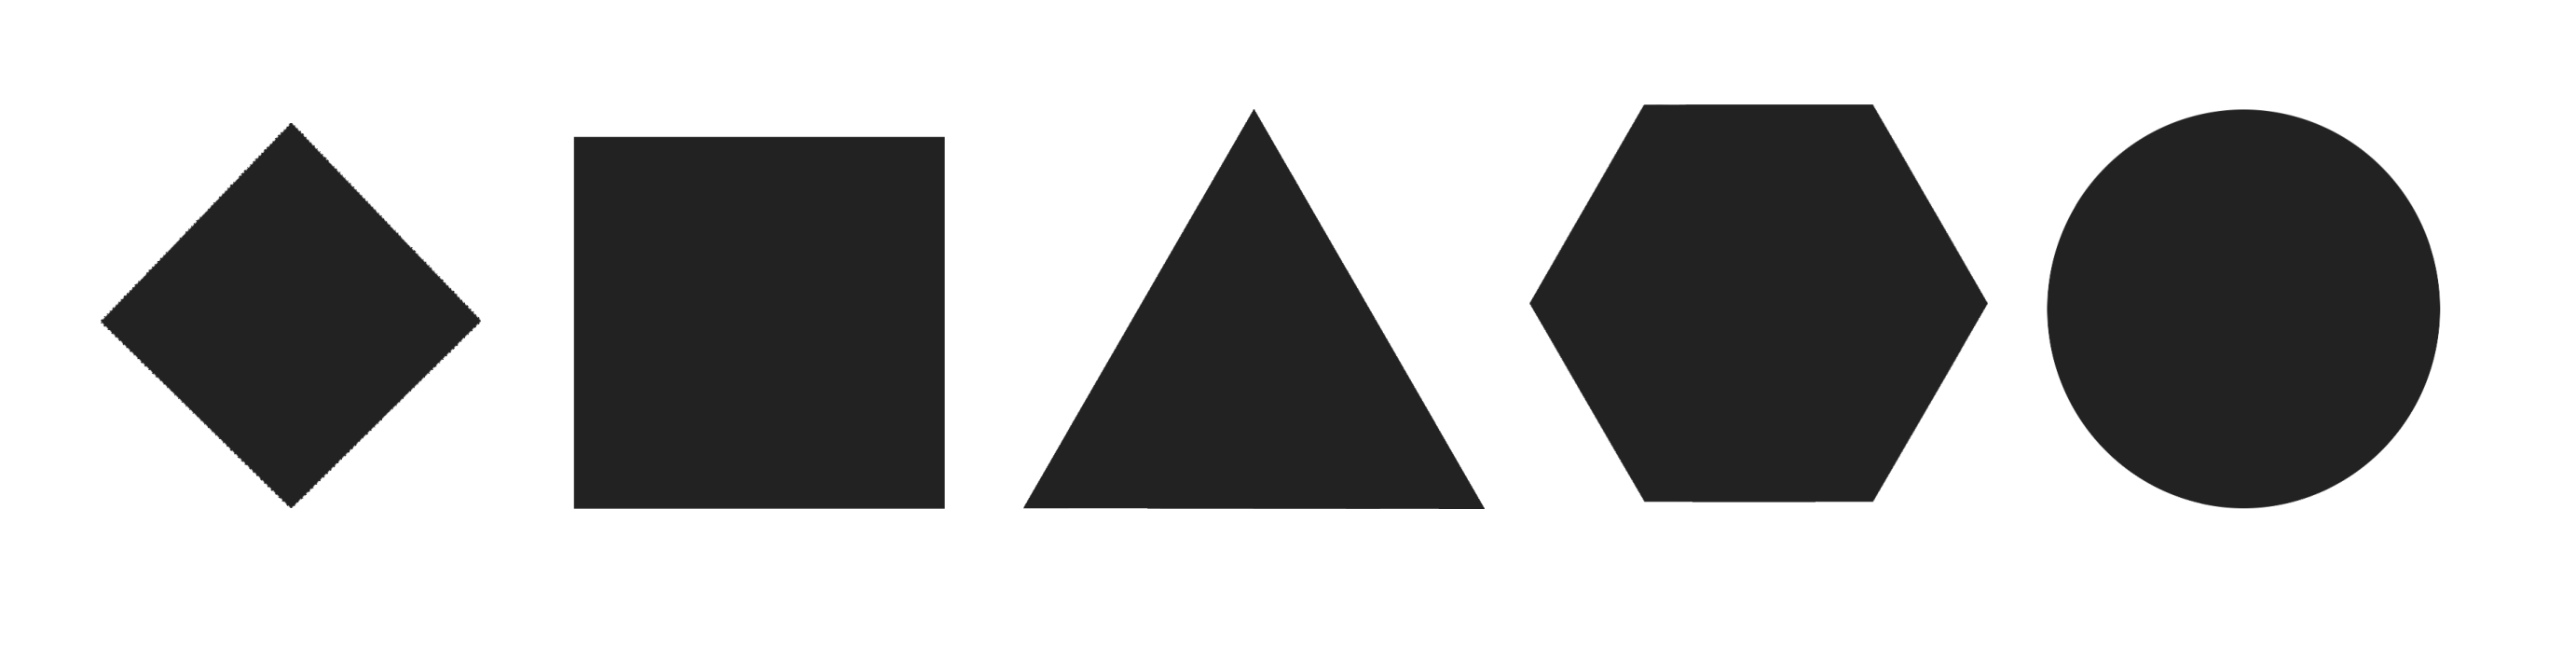
\includegraphics[scale=0.15]{figures/experiment_2_stimuli.pdf}
  \end{center}
\end{figure}

\subsubsection*{Procedure}

\begin{table}[!ht]
  \begin{center}
    \caption{Abstract design of Experiment 2 including both test and training phases. X and Y are in place of the category labels. During the test phase, participants needed to select either X or Y to complete the features shown below.\\}
    \label{tab:abstract-exp2}
    \begin{tabular}{llr} % text alignments
      \textbf{Training (Relative Frequencies)} & \textbf{Test}& \\
      \hline
      % & \\
      ABX x 3 &  A, B, C,         &  \\
      ACY x 1 &  AB, AC, BC      & x 20 \\
      \hline
    \end{tabular}
  \end{center}
\end{table}


\subsection{Results and Discussion}

30 made it into the analysis

\begin{table}[H]
  \begin{center}
    \caption{Caption.\\}
    \label{tab:results-exp2}
    \vskip 0.12in
    \begin{tabular}{rcc}
      \hline
       & $P(common)$ & $P(rare)$ \\
      \hline
      A & 0.78 & 0.22  \\
      AB & 0.95 & 0.05 \\
      AC & 0.09 & 0.91 \\
      B & 0.92 & 0.07  \\
      \textbf{BC} & \textbf{0.35} & \textbf{0.65} \\
      C & 0.08 & 0.92 \\
    \end{tabular}
  \end{center}
\end{table}

$M = 0.64$, 95\% HDI $[0.53, 0.75]$, $\mathrm{BF}_{10} = 4.09$

\section{Discussion}

- asymmetric representation as an assumption

Asymmetric representation can arise in different ways.
One way it is manifested is the attentional tuning of cognitive representation of category exemplars.
Another scenario is

- auxiliary phenomenon (Wills CIRP addition)
- Things that any theory of IBRE should explain
- current theories fall short
- eye-tracking and attention

\section{Open Science}

\section{Acknowledgments}

In the \textbf{initial submission}, please \textbf{do not include
  acknowledgments}, to preserve anonymity.  In the \textbf{final submission},
place acknowledgments (including funding information) in a section \textbf{at
the end of the paper}.

\bibliographystyle{apacite}

\setlength{\bibleftmargin}{.125in}
\setlength{\bibindent}{-\bibleftmargin}

\bibliography{library}


\end{document}
